
\label{sec:systemArchitecture}

Dieses Kapitel soll ein Gefühl für die Komponenten von \emph{Flewnit} und 
ihre Zusammenhänge vermitteln. Die Komponenten "`in Aktion"' werden im Detail im Verlauf des Kapitels 
\ref{sec:simulation} beschrieben.

Das System wurde in C++ als (wahlweise statisch oder dynamisch zu linkende) Bibliothek implementiert.
Der Code der GPU-Programme ist in GLSL bzw. OpenCL C verfasst.

\subsection{Dependencies}
	\label{sec:dependencies}
	
	Zunächst sollen die verwendeten Third-Party-Bibliotheken kurz vorgestellt werden:

	\begin{description}
		\item[OpenGL3/4]
		Die schon mehrfach erwähnten modernen Versionen der \linebreak \emph{Open Graphics Library},
		der offenen API der Khronos Group zur \linebreak hardwarebeschleunigten Graphik-Programmierung 
		auf Basis der Dreiecks-Rasterisierung.
		\todo[color=green]{evtl treffenderen Ausdruck finden: Scanline-basiert oder was auch immer}
		Um die Programmierung ohne Legacy-Routinen nicht erst zur Laufzeit über einen OpenCL-Error
		durch Verwendung eines Core-Profiles zu erzwingen, gibt es einen OpenGL- Header
		namens "`gl3.h"'\footnote{beziehbar unter http://www.opengl.org/registry/},
		der in Kombination mit der entsprechenden Präprozessor-Definition
		\lstinline[language=C]|#define GL3_PROTOTYPES 1| schon zur Compile-Zeit nur die non-deprecated
		Routinen zur Verfügung stellt.
		
     	\item[OpenCL 1.0]
	    Die \emph{Open Computing Language}, erste Version der noch jungen API für massiv parallele Programmierung
	    \footnote{die GPGPU-Computing einschließt}, wie OpenGL von der Khronos Group verwaltet; 
	    sie stellt den ersten offenen Standard für GPGPU dar, d.h., die Verwendung der API ist nicht mehr an eine
	    bestimmte Hardware (wie bei Nvidia CUDA) oder ein bestimmtes Betriebssystem (wie Microsofts DirectCompute)
	    gebunden.
	    
	    Zur Zeit der Implementierung waren noch keine Non-Developer-Treiber für OpenCL 1.1 verfügbar, 
	    außerdem gab es kein Feature dieser Version, welches ich dringend benötigt hätte.
	    Deshalb habe ich die Version 1.0 verwendet.
	    
	    Es gibt einen C++ -Wrapper der C-API, welcher stark auf C++-Templates basiert und in einer einzigen Headerdatei 
	    implementiert ist. Dieser ist direkt von der Khronos-Homepage\footnote{http://www.khronos.org/registry/cl/} 	
	    beziehbar. Diesen Wrapper habe ich verwendet, da er die Nutzung der API wesentlich eleganter macht.
	    
    	
   		\item[GLFW 2.7]
		Wie auf Seite \pageref{focus:dependencies} angedeutet, waren mir folgende Dinge wichtig, damit die Einsetzbarkeit
		des Frameworks in professionelleren Kontexten nicht schon im Vorfeld verbaut ist:
		\begin{itemize}
			\item Option auf Fullscreen
			\item Option auf Multisampling
			\item Die Möglichkeit der Erstellung eines OpenGL-Kontextes einer frei wählbaren Version 
			mit Option zwischen Core- und Compatibility-Profile
			\item Option auf "`\emph{Mouse Grab}"', so dass man wie in einem Computerspiel mit ausgeblendetem Mauszeiger
			nur durch Bewegung der Maus ohne Bildschirm-/Fenster-Grenzen die virtuelle Kamera rotieren kann;
			\item "`Input events"', d.h. Aktualisierungen von Benutzereingaben sollen häufig und mit minimaler 
			Latenz geschehen, außerdem so unabhängig wie möglich von der Framerate sein;
			Nach möglichkeit sollten Input-Updates zumindest "aktiv abfragbar" sein 
			(im Gegensatz zum passiven Warten darauf, dass von der Input-Library eine Callback-Funktion 
			aufgerufen wird)
			\item Es soll volle Kontrolle über die "Render-Loop" geben, so dass man nicht 
			den Kontrollfluss an eine Funktion übergibt, die womöglich nie zurückkehrt und weiteren Kontrollfluss
			durch das Benutzerprogramm	nur über Callback-Funktionen ermöglicht
			(wie \lstinline[language=C]|glutEnterMainLoop()| beim in die Jahre gekommenen \emph{GLUT}).
			Ein derartiges Konstrukt ist einer
			Engine nicht würdig und verhindert womöglich sauberes Herunterfahren und Neu-Initialisierung,
			wie es z.B. beim Wechseln einer Szene oder eines fundamentalen globalen Settings nötig sein könnte.	
		\end{itemize}
		\emph{GLFW}\footnote{http://www.glfw.org/} in der Version 2.7, die zum Zeitpunkt der Implementation aktuellste 
		stabile	Version, erfüllt diese Forderungen, und findet damit in \emph{Flewnit} Einsatz sowohl im Fenster- als auch 	
		im Input-Manager. Die Timing-Funktionalität wird ebenfalls von GLFW übernommen.
		
    	
    	\item[OpenGL Mathematics (GLM)]
    	Seit sämtlicher Mathematik-bezogener OpenGL-state inklusive zugehöriger built-in-Variablen und -Funktionen
    	wie \lstinline[language=GLSL]|gl_ModelViewProjectionMatrix| oder
    	\lstinline[language=GLSL]|ftransform()|
    	in GLSL abgeschafft wurden, führt um eine Bibliothek für Vektor- und Matrix-Algebra kein Weg mehr herum.
    	Ich habe mich für \emph{GLM}\footnote{http://glm.g-truc.net/} entschieden, da sie klein und dennoch mächtig ist,
    	mit einigen Convenience-Functions; QT hat ebenfalls eine Mathe-Bibliothek, verwendet jedoch
    	\lstinline[language=C]|double|, also 64bit-Fließkomma-Werte als Basis-Datentyp, was das direkte Übergeben
    	als Array von \lstinline[language=C]|float|-Uniforms an die OpenGL-Shader verhindert. Zwar unterstützen OpenGL
    	und moderne Graphikkarten \lstinline[language=C]|double| nativ, jedoch mit drastisch geringerer Geschwindigkeit,
    	da weniger Recheneinheiten für diesen Datentypen zur Vervügung stehen.
    	Es sei bemerkt, dass ich persönlich die direkte Verwendung einer C++ - Mathe-Bibiothek mit überladenen Operatoren
    	und eigener Akkumulation von Matrizen wesentlich angenehmer und eleganter finde als das zähe Hantieren
    	mit dem C-API zum modifizieren des OpenGL-State mit seinen Matrix-Modes.
    	
    	\item[Grantlee]
       		Die bereits erwähnte Template- Engine; die Syntax entspricht der der Template-Sprache des 
       		\emph{Django} web Frameworks\footnote{https://www.djangoproject.com/}.
       		Die Engine stellt einen Vererbungs-Mechanismus bereit:\\
       		Auf diese Weise kann z.B. die Datei "`particleSimulationTemplate.cl"' verschiedene "`Code-Blocks"'
       		definieren wie z.B.
       		\lstset{language=GLSL} 
       		\begin{lstlisting}

	
	the core of the physics simulation: 
	accumulate all relevant values 
	(density, pressure force, viscosity force etc ...)
	               

       		\end{lstlisting}
       		, die von anderen Datein geerbt und entsprechend angepasst implementiert werden.\\
       		"`updateDensity.cl"' erbt von dieser Datei durch die Directive
       		\lstinline[language=GLSL]|| 
       		und implementiert die Dichte-Berechnungen, 
       		ohne dass der umschließende (nicht unerheblich lange und komplexe) Kontrollfluss-Code wiederholt werden muss:
       		\begin{lstlisting}

	if( BELONGS_TO_FLUID(
			GET_CURRENT_NEIGHBOUR_PARTICLE_OBJECT_ID  ) )
	{
		ownDensity +=                   
			cObjectGenericFeatures [ GET_CURRENT_NEIGHBOUR_PARTICLE_OBJECT_ID  ].massPerParticle
			* poly6( ownPosition -  GET_CURRENT_NEIGHBOUR_POS , cSimParams );
	}

       		\end{lstlisting}

       		
       		
    	\item[Assimp]
    	Die \emph{Open Asset Import Library}\footnote{http://assimp.sourceforge.net/} ermöglicht das Auslesen
    	von Szenen direkt aus .blend-Dateien, dem nativen Datenformat des exzellenten Free Software -- 3D-
    	Modellierungsprogramms \emph{Blender}\footnote{http://www.blender.org/}.
    	Somit entfällt der Umständliche Export in ein Zwischenformat.

    	
   		\item[TinyXML]
   		Um zu gewährleisten, dass das System schon in der frühen Entwicklungsphase weitgehend ohne 
   		Recompile-benötigenden "`Hard-Codes"' konfigurierbar ist, wurde TinyXML verwended, um eine XML-
   		config-Datei zu parsen.    	
    
	
	\end{description}	

	Außerdem haben manche Komponenten der \emph{Boost}-Libraries\footnote{http://www.boost.org/} verwendet.
	
	


\subsection{Klassendiagramm}
Abbildung \ref{fig:ClassDiagOverview1} und \ref{fig:ClassDiagOverview2} zeigen ein vereinfachtes Klassendiagramm
von \emph{Flewnit}. Die roten Klassen stellen wichtige Meta-Informationen dar, um Kontrollfluss und Objekt-Erstellung
zu delegieren. In den folgenden Unterabschnitten werden die einzelnen Komponenten detaillierter vorsgestellt.

\begin{figure}[!h]
	 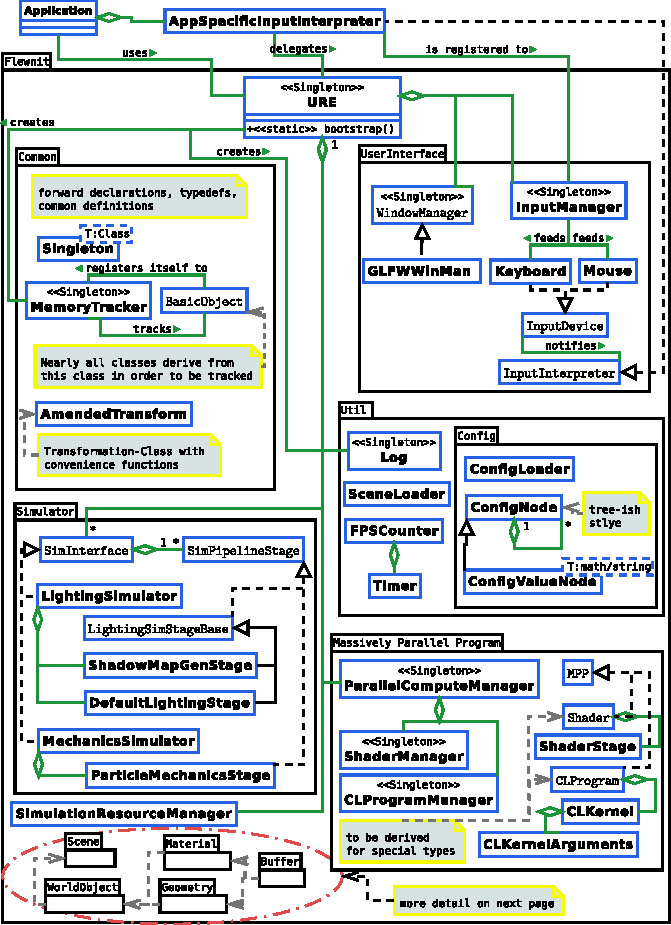
\includegraphics[width=1.15\textwidth]{Overview_Flewnit_Architecture_After_Implementation1.pdf}
	\caption{Klassendiagramm des Gesamtsystems, Teil 1}
	\label{fig:ClassDiagOverview1}
\end{figure}


\begin{figure}[!h]
	 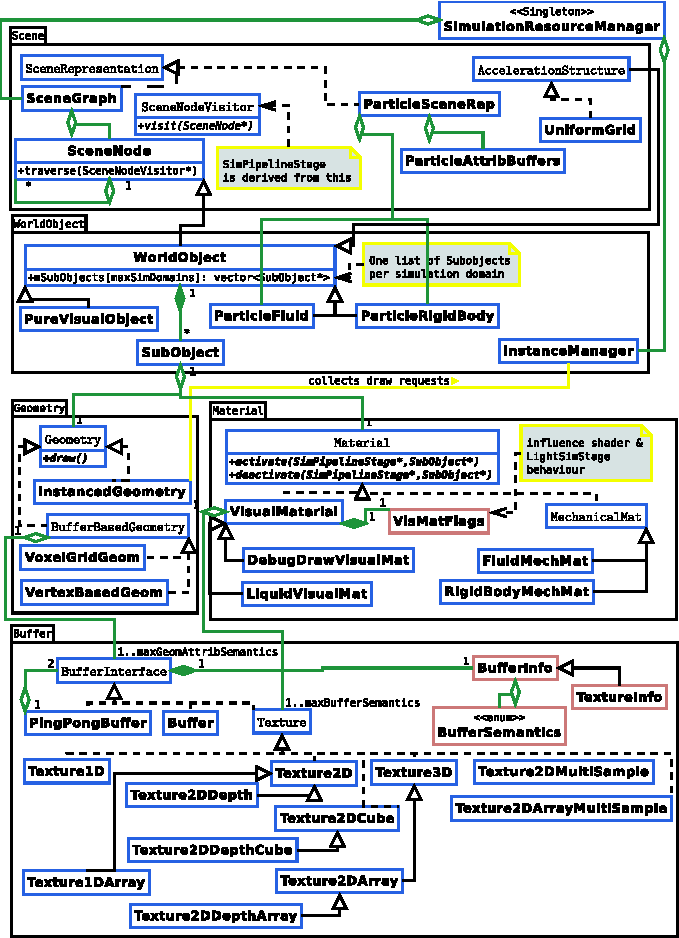
\includegraphics[width=1.15\textwidth]{Overview_Flewnit_Architecture_After_Implementation2.pdf}
	\caption{Klassendiagramm des Gesamtsystems, Teil 2}
	\label{fig:ClassDiagOverview2}
\end{figure}



 
\subsection{BasicObject und Memory Tracking}
	\lstset{language=C++} %we want c++ code listings
	
	Die Bibliothek soll zur Laufzeit kontrolliert herunterfahr- und re-initialisier-bar sein, 
	um eine vielseitige und flexible Anwendung zu gewährleisten. Da bei C++ das Speicher-Management dem
	Programmierer überlassen ist, und man daher vor allem bei massiver Nutzung von Pointern schnell den Überblick
	verliert, 
	\begin{itemize}
		\item welches Objekt welche anderen erschaffen hat
		\item welche Objekte eine Klasse "`besitzt"' und somit für ihre Speicher-Freigabe zuständig ist bzw
		\item auf welche Objekte eine Klasse nur ein Handle für Verwaltung oder	Backtracking hat, ohne für Erschaffung
		 oder Löschung zuständig zu sein
	\end{itemize}
	wurde in Anbetracht der oberen Forderung ein sehr simples Meta-Object-System system realisiert, welches Klassen-Namen
	und Speicherverbrauch eines Objektes feststellt sowie jedem Objekt eine \emph{unique ID} zuweist.
	Zweck dieses Meta Object System-Systems war es, Speicherlecks durch Nicht-Löschen von Objekten während der Entwicklung 
	zu finden;
	
	Dafür erbt beinahe jede Klasse in \emph{Flewnit} von \lstinline|BasicObject|.
	Diese Klasse registriert sich automatisch bei der \lstinline|MemoryTracker|-Singleton-Instanz, bekommt dort eine
	ID zugewiesen. Diese ID hat noch keine Anwendung, könnte sich aber in einem Netzwerk-Kontext als nützlich erweisen.

	Wie bei Qt das \lstinline[language=C++]|Q_OBJECT|-Makro muss in jede von 
	\lstinline[language=C++]|BasicObject| erbende Klasse das Makro 
	\lstinline[language=C++]|FLEWNIT_BASIC_OBJECT_DECLARATIONS| eingetragen werden; Dieses Makro definiert die 
	Implementatoin einer virtuellen Funktion, welche die Meta-Information setzen:
    \begin{lstlisting}
#define FLEWNIT_BASIC_OBJECT_DECLARATIONS \
	public:\
		virtual void initBasicObject() \
		{ \
			mMemoryFootPrint = (int) sizeof(*this); \
			mClassName = String(typeid(*this).name()); \
		} \
	private:	
	\end{lstlisting}
	Diese umständliche Implementierung hat die Urasache, dass Typ-Informationen der Blatt-Klasse einer
	Klassenhierarchie erst dann zur verfügung stehen, wenn alle Konstruktoren der Basis-Klassen zurückgekehrt sind,
	weshalb der obere Code also nicht im Konstruktor der Basisklasse stehen darf, da der \lstinline|this|-Pointer
	noch nicht die Informationen der Blatt-Klasse enthält.
	Ferner, um dem Programmierer nicht zuzumuten, \lstinline|initBasicObject()| in jedem Konstruktor aufzurufen
	(das führt bei tiefen Klassenhierarchien zu unnötigen ausführungen dieser Funktion, da nur die Info der Blatt-Klasse
	benötigt wird, außerdem entstünde so eine weitere Vergesslichkeits-Fehlerquelle, die durch das Meta Object System ja 
	gerade \emph{vermieden} werden soll), stellt der Memory Tracker eine Routine \lstinline|updateMemoryTrackingInfo()|
	bereit, die aufgerufen werden sollte, wenn man auf valide meta-Information zugreifen will.
	
	Über bedingte Kompilierung lässt sich diese Meta-Funktionalität deaktivieren.
	Ein "`richtiges"' Meta Object System wie das von Qt wollte ich nicht verwenden, da es für meine Zwecke zu komplex und
	mächtig ist, und ich nicht mit Kanonen auf Spatzen schießen wollte. Ohnehin gibt es Tools wie Valgrind, mit denen
	man Speicherlecks finden kann. 

	Letztendlich ist meine Lösung nicht wirklich elegant (auch wenn ich ohne Meta-Object-Compiler (MOC) keine bessere 	
	Lösung gefunden habe) und daher eher als eine Spielerei anzusehen
	mit dem Zwecke, die C++-Interna zu verinnerlichen und zu jeder Zeit daran erinnert zu werden, 
	Destruktoren zu implementieren und sich über 
	"`Besitz- und Verwaltungs-Verhältnisse"' der Klassen Gedanken zu machen.
	
	Der \lstinline|MemoryTracker| verfolgt auch sämtliche Allokationen der \lstinline|BufferInterface|-Klasse,
	also der Basisklasse sämtlicher Buffer-Typen;
	
\subsection{AmendedTransform}
 	Im Zuge der Überlegungen zum Szenegraphen, der Kamera und des visuellen Renderings vieler Objekte per
 	Hardware-Instancing entschied ich mich, die klassische 4x4-Transformationsmatrix zu wrappen und mit
 	convenience functions anzureichern, siehe Listing \ref{listing:AmendedTransformDef}.\\
 	Der Zweck dieser Klasse ist es, Transformationsmatrizen anhand "`anschaulicher"' Parameter 
 	(Position, Richtung, Up-Vektor, Skalierung) zu definieren,
 	und diese Parameter auch nach Akkumulationen, Modifikationen und/oder Animationen zur Verfügung zu haben.\\
 	Der Fokus liegt hier klar auf der Bequemlichkeit für den Entwickler, nicht auf der Performanz.
 	Sobald sehr große, dynamisch animierte und tiefe Scenegraphen zum Einsatz kommen, könnte diese Klasse
 	zum Flaschenhals werden. Dann ist vielleicht ein Refactoring vonnöten; Vorerst scheint mir die Implementation jedoch
 	angemessen.\\
 	
 	Auf diese Weise lässt sich z.B. bequem ein \lstinline|Camera|-Objekt, welches selber von \lstinline|WorldObject| erbt,
 	welches wiederum von \lstinline|SceneNode| abgeleitet ist, an eine andere SceneNode anhängen, und aus der automatisch
 	berechneten globalen Transformation erhält man durch \lstinline|AmendedTransform::getLookAtMatrix()|
 	direkt die lookAt-Matrix;
 	Auch typische Animationen werden von der Klasse übernommen. Ob dies guter Stil ist, oder doch lieber in die
 	SceneNode-Klasse ausgelagert werden sollte, ist eine Frage, die ich noch nicht abschließend beantworten kann.
 	Eine Erötertung lasse ich aus, da das Refactoring in diesem Falle nicht zu aufwändig wäre;

	Es sei bemerkt, dass durch die Menge an Matrizen, die an den Vertex Shader beim Instanced Rendering übergeben
	werden müssen... \todo[color=green]{normal matrix erklaeren, nonuniform scaling verboten etc.}
 	
 	\begin{lstlisting}[caption={AmenededTransform Klassendefinition, gekürzt},label=listing:AmendedTransformDef]
class AmendedTransform
{
public:
	AmendedTransform(
			const Vector3D& position = Vector3D(0.0f,0.0f,0.0f),
			//(0,0,-1) is assumed as initial orientation, extress any deviation in euler angles(radians)
			const Vector3D& direction = Vector3D(0.0f,.0f,-1.0f),
			const Vector3D& upVector = Vector3D(0.0f,1.0f,0.0f),
			float scale = 1.0f);
	AmendedTransform(const AmendedTransform& rhs);
	virtual ~AmendedTransform();

	AmendedTransform operator*(const AmendedTransform& rhs)const;
	const AmendedTransform& operator*=(const AmendedTransform& rhs);
	const AmendedTransform& operator=(const AmendedTransform& rhs);

	//accum: translationMatrix * rotationMatrix * scaleMatrix;
	const Matrix4x4& getTotalTransform()const;
	//convenience functions:
	//unscaled, i.e. orthonormal rotation matrix:
	Matrix3x3 getRotationMatrix()const;
	//inverse of (translationMat*rotationMat);
	Matrix4x4 getLookAtMatrix()const;
	Matrix4x4 getScaleMatrix()const;
	Matrix4x4 getInverseScaleMatrix()const;
	static bool matricesAreEqual(const Matrix4x4& lhs, const Matrix4x4& rhs);
	AmendedTransform getInverse()const;

	/*... getter and setter for pos, dir, up omitted */ 

	//"animation" functions:
	void moveRelativeToDirection(float forwardBackward, float rightLeft, float upDown);
	//change direction by rotating it angleDegrees degrees around cross(direction,upVector)
	void pitchRelativeToDirection(float angleDegrees);
	//change direction by rotating it angleDegrees degrees around the upVector;
	void yawRelativeToUpVector(float angleDegrees);

protected:
	//backtrace pointer to tell the scene node to update itself after its transform has been modified directly;
	//mOwningScenNode->transformChanged(bool global) will be called by any setter function of this class if there is an
	//associated SceneNode;
	SceneNode* mOwningSceneNode;
	//flag needed by Scene node to update itself appropriately
	bool mIsGlobalTransform;
	
	friend class SceneNode;
	void setOwningSceneNode(SceneNode*node, bool isGlobalTransform)
		{mOwningSceneNode = node; mIsGlobalTransform=isGlobalTransform;}


	Vector3D mPosition;
	Vector3D mDirection;
	Vector3D mUpVector;
	float mScale;
	
	Matrix4x4 mAccumTranslationRotationScaleMatrix;

	//construct the transformation matrix from current pos,dir,up,scale; is called by any related setter;
	//validates members, if possible
	void setup();

	//protected matrix-constructor to omit that the user passes a non-conforming matrix	
	AmendedTransform(const Matrix4x4& transform);
	friend class Loader;//the loader may set transformation matrices ;)
};
 	\end{lstlisting}
    	
    	
    	
\subsection{Die \emph{Unified Rendering Engine}}
URE blubb

\subsection{Die Simulator-Klassen}

	Camera, Light, RenderTarget: alles WorldObjects


\subsection{Die SimulationPipelineStages}
	shdow map gen, direct lighting, rendering features particlemechanics stage;
	in planung: deferred rendering G-Bufferfill, deferred rendering shade, div. post processing stages


\subsection{Die Manager-Klassen}
Für gemeinsamen zugriff sollten viele Daten für andere Klassen verfügbar sein (Buffer, Rendering Results...); 	
Realisierung über Manager-Singleton-Klassen und Zugriff über Map-Container;
\todo[color=green]{evtl. andere reihenfolge}

\subsection{Die Template-Engine}
	\label{sec:architecture:templateEngine}
	exemplarischer code schnipsel, refernz su shadermanager und CLProgramManager, erklärung wie man templat contex setzt, 	
	vererbung etc;
    	
\subsection{Die Buffer-Abstraktion}  
	\label{sec:architecture:BufferAbstraction} 	
 	die bombe, die cpu, ogl und ocl vereint, inclusive ping ponging etc.. 
 	fundamentale Klassensammlung fuer den Unified-Aspekt
 	
 	\begin{figure}[!h]
  		\begin{tabular}
  		{
  		 l  l | c | c | c |
  		}
																	\cline{3-5}
  									&								&	\multicolumn{3}{ c | }{Context} \\ 
  																	\cline{3-5}
									&								& 	Host 	& 	OpenGL 	& 	OpenCL	\\
    	\noalign{\hrule}								
    	\multicolumn{1}{|c|}{
    		generic Buffer
    	}							& 								
    		&	{\color{green}\checkmark} 	&	{\color{red}x}		& 	{\color{green}\checkmark}	\\ 
    	
    	\noalign{\hrule}								
    	\multicolumn{1}{|c|}{
    		\multirow{4}{*}{OpenGL Buffers}
    	}							& Vertex Attribute Buffer		
    		&	{\color{orange}o} 	&	{\color{green}\checkmark}		& 	{\color{orange}o}	\\  
    								\cline{3-5}
    	\multicolumn{1}{|c|}{}		& Vertex Index Buffer			
    		&	{\color{orange}o} 	&	{\color{green}\checkmark}		& 	{\color{orange}o}	\\  
    								\cline{3-5}
    	\multicolumn{1}{|c|}{}		& Uniform Buffer
    		&	{\color{orange}o} 	&	{\color{green}\checkmark}		& 	{\color{orange}o}	\\ 
    								\cline{3-5} 
    	\multicolumn{1}{|c|}{}		& Render Buffer					
    		&	{\color{red}x} 	&	{\color{green}\checkmark}		& 	{\color{green}\checkmark}	\\ 
    
   		\noalign{\hrule}								
   		\multicolumn{1}{|c|}{
    		\multirow{4}{*}{Textures} 
   		}							& 1D Texture					
   			&	{\color{orange}o} 	&	{\color{green}\checkmark}		& 	{\color{red}x}	\\ 
    								\cline{3-5}
		\multicolumn{1}{|c|}{}		& 2D Texture				
			&	{\color{orange}o} 	&	{\color{green}\checkmark}		& 	{\color{green}\checkmark}	\\ 
									\cline{3-5}
		\multicolumn{1}{|c|}{}		& 3D Texture		
			&	{\color{orange}o} 	&	{\color{green}\checkmark}		& 	{\color{green}\checkmark}	\\ 
									\cline{3-5}
		\multicolumn{1}{|c|}{}		& Special Texture				
			&	{\color{orange}?} 	&	{\color{green}\checkmark}		& 	{\color{orange}?}	\\ 


    	\noalign{\hrule}
     
     	
  		\end{tabular}	
  	
  		\caption{		
  			Verschiedene Buffertypen und ihre Verfügbarkeit in verschiedenen Kontexten \\	
  			Legende: \\
			{\color{green}\checkmark}	$\rightarrow$ nativ unterstützt;
			{\color{orange}o}	$\rightarrow$ kompatibel;
			{\color{red}x}	$\rightarrow$ nicht unterstützt;	\\
			{\color{orange}?}	$\rightarrow$ Unterstützung abhängig von weiteren Parametern;	
		}
	
  	\end{figure}
 
\subsection{Das WorldObject}
	Basis-Klasse fuer alles was unified simuliert wird: pure viuelle objekt, uniform grid, fluid, rigid body etc..
	
	\subsubsection{Das SubObject}
  
 
\subsection{Material}  
	was stellt welches material in welcher Domain dar?
	
\subsection{Geometry}
	Abtract, Buffer based, Vertex based etc.. ein paar konzepte (implementiert/genutzt nur VertexBased)  
	
\subsection{Massively Parallel Program}
	Basisklasse von Shader und OpenCL Program
	\subsubsection{Shader}
		
	\subsubsection{OpenCLProgram}

weitere klassen/konzepte to go...	


\subsection{Status der Implementierung am Ende der BA}
	
	Features auflisten;
	\todo[color=green]{screenshots? oder lieber erst später,zusammen mit detaillierter erläuterung?}

	großteils programmierte, aber ungenutzte/ungetestete features erwähnen (Deferred Rendering, Layered Rendering, 	
	RenderTarget-Klasse, Partikel-Rigid bodies, verschiedene Fluid-Typen); 


	überlegte aber nciht programmierte Konzepte/Algorithmen erwähnen (Triangle-Index-Voxelisierung)
	
	schlimmste schnitzer nennen, wie
		- miese fluid-visualisierung, 
		- unübersichtliche shadertemplates, besser gemacht bei CL-
			Kernel-Templates, 1. weil struktur hier besser "vererbbar", 2. weil mehr erfahrung mit  Template-Engine
	
	  	
  	

\clearpage
